\section{Grafiken}

\subsection{Verschiedene Möglichkeiten}

Nun werden Grafiken eingefügt auf verschiedenste Weise.\\
Wie in der Abbildung \ref{fig:test_plot_1} zu sehen ist.

\begin{figure}[!ht]
\centering
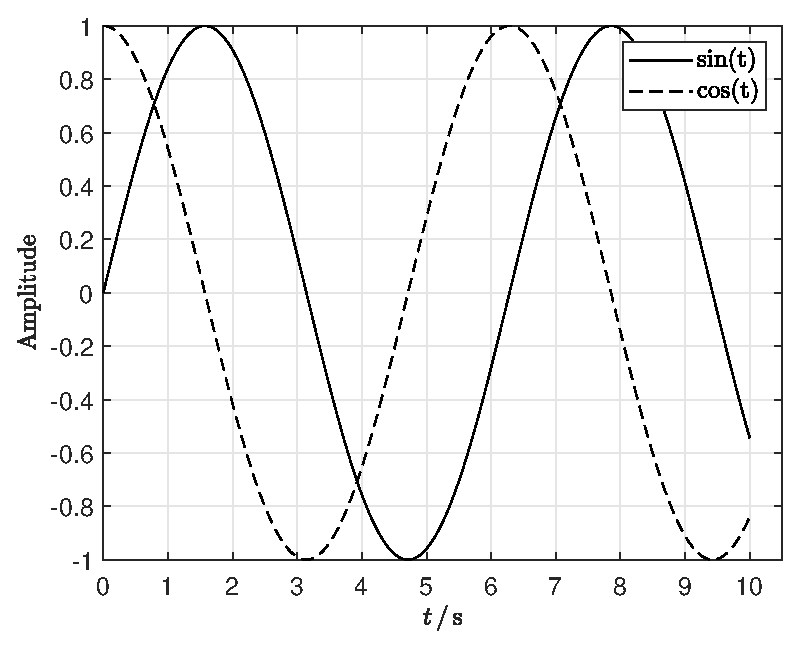
\includegraphics[width=0.6\textwidth]{Plot/Test_plot_1.eps}
\caption[60\,\% der Textbreite]{Sinus- und Cosinus-Verlauf über die Zeit dargestellt.\cite{Sensoren}}
\label{fig:test_plot_1}
\end{figure}

\begin{figure}[!ht]
\centering
\input{Plot/test.tikz}
\caption{mit .tikz gemacht}
\label{fig:myfirstfig}
\end{figure}

\clearpage
Die nächsten zwei Abbildungen (\ref{fig:subhouse21} und \ref{fig:subhouse22}) zeigen jeweils eine Möglichkeit zwei Grafiken nebeneinander einzufügen.\cite{Sensoren}
\begin{enumerate}
    \item Bei der Ausrichtung stehen der Möglichkeiten zur Auswahl: c (für Center) t (für Top) und b (für Bottom)
    \item Mit diesem folgenden Befehl kann das Bild skaliert werden \glqq\textit{keepaspectratio}\grqq{} und nach einem Anführungszeichen sollte immer ein Leerzeichen eingefügt werden mit einem Backslash, oder mit zwei geschwungenen Klammern.
\end{enumerate}

\begin{figure}[!ht]
\centering
\input{Plot/test.tikz}
\caption[]{Sinus- und Cosinus-Verlauf über die Zeit dargestellt.}
\label{fig:myfirstfi}
\end{figure}

\clearpage
\begin{figure}[!ht]
    \begin{subfigure}[b]{.48\textwidth}
    \centering
    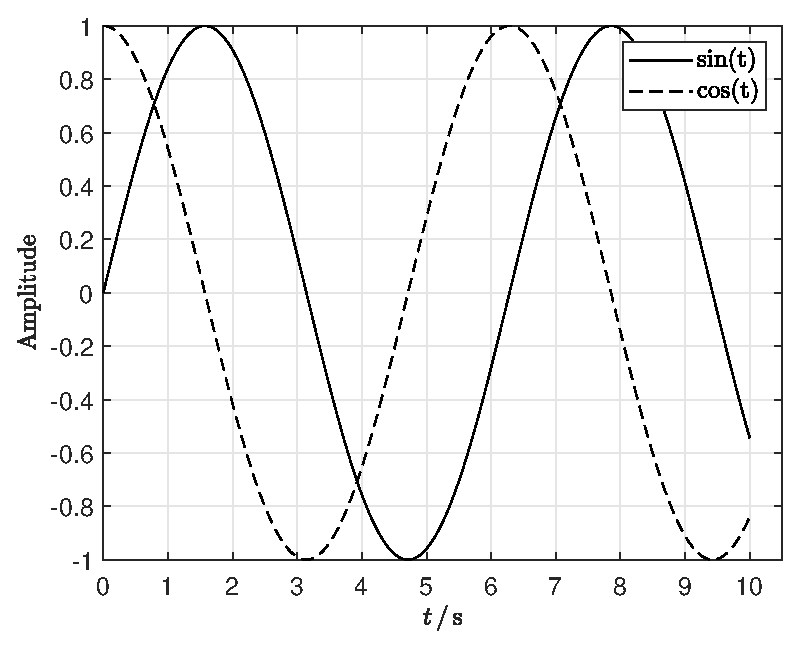
\includegraphics[width=0.95\textwidth]{Plot/Test_plot_1.eps}
    \caption{erster Affe}
    \label{fig:subhouse21}
    \end{subfigure}
\hfil
    \begin{subfigure}[b]{.48\textwidth}
    \centering
    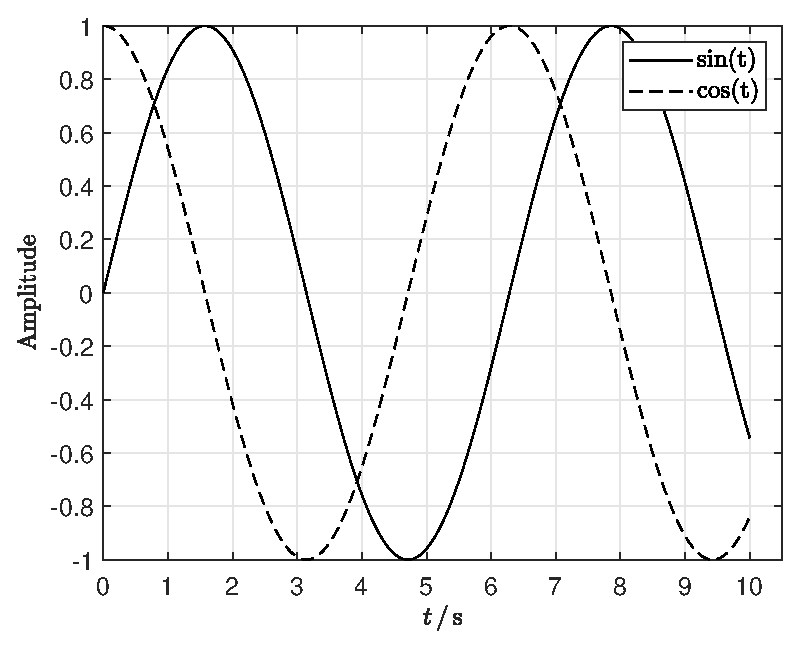
\includegraphics[width=0.95\textwidth]{Plot/Test_plot_1.eps}
    \caption{zweiter Affe}
    \label{fig:subhouse22}
    \end{subfigure}
\caption[zwei Pferde]{\centering Die Nebenstehenden Bilder sollten nach diesen Schema eingefügt werden. (Steht im Loborleitfaden)}    
\label{fig:Doppelbild}
\end{figure}

\subsection{Bild und nebenbei eine Tabelle}
\begin{figure}[!ht]
    \begin{subfigure}[b]{.48\textwidth}
    \centering
    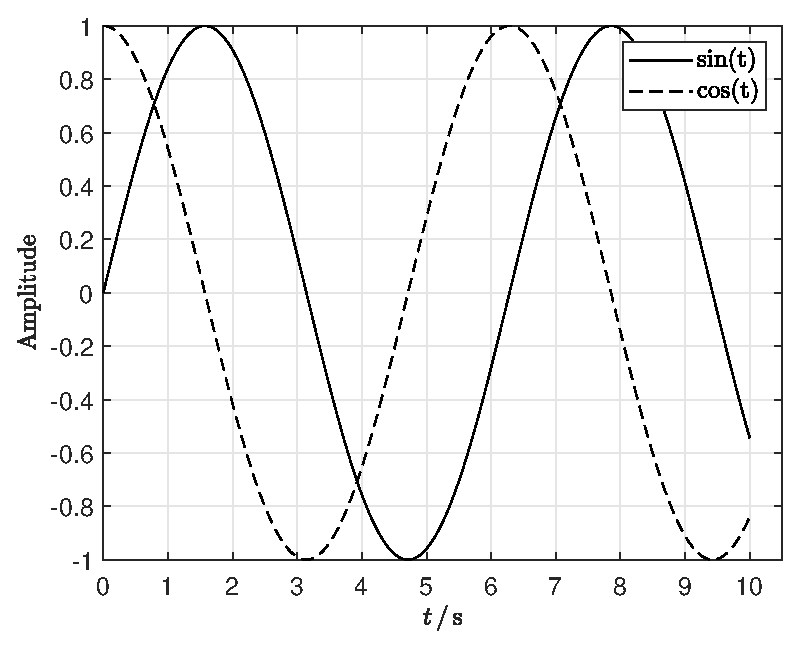
\includegraphics[width=0.95\textwidth]{Plot/Test_plot_1.eps}
    \caption{erster Affe}
    \label{fig:subhouse23}
    \end{subfigure}
\hfil
    \begin{subfigure}[b]{.48\textwidth}
    \centering
    \resizebox{0.95\textwidth}{!}{
    \begin{tabular}{*{3}{c}}
        \hline
            Beschreibung & Abkürzung & Größe \\
        \hline
            Statische Verstärkung & $K$ & $0.71$\\
            Zeitkonstante 1 & $\tau_1$ & $0.24$\,\si{\second}\\
            Zeitkonstante 2 & $\tau_2$ & $0.68$\,\si{\second}\\
    \end{tabular}
    }
    \caption{zweiter Affe}
    \label{tab:subhouse123}
    \end{subfigure}
\caption[Zwei Schweine]{Zwei Affen}
\label{fig:subhouses2}
\end{figure}

So und jetzt ist genug mit den Grafiken, weiteres werden Tabellen erstellt bevor zu den mathematischen Formeln gewechselt wird. 
\clearpage

\section{Tabellen}


Verschieden bsp. Tabellen werden

\begin{table}[htp]
\renewcommand{\arraystretch}{1.2} %% Abstand zwischen den Zeilen wird größer
\centering
\caption[Vorgegebene Größen]{Vorgegebene Größen}
\label{tab: Vorgegebene Größen}
\footnotesize
%\resizebox{.6\textwidth}{!}{
\begin{tabular}{*{3}{c}}
    \toprule
    Beschreibung & Abkürzung & Größe \\
    \midrule
    Versorgungsspannung & $U_b$ & $20$\,\si{\volt}\\
    Eingangsspannung & $U_{ein}$ & $\pm0.5$\,\si{\volt}\\
    Ausgangsspannung & $U_{aus}$ & $\pm5$\,\si{\volt}\\
    Untere Grenzfrequenz & $f_{gu}$ & $100$\,\si{\hertz}\\
    Obere Grenzfrequenz & $f_{go}$ & $10$\,\si{\kilo\hertz}\\
    Eingangswiderstand & $R_{ein}$ & $10$\,\si{\kilo\ohm}\\
    Lastwiderstand & $R_{aus}$ & $10$\,\si{\kilo\ohm}\\
    \bottomrule
    \end{tabular}
%}    
\end{table}



\begin{table}[htp]
\centering
\caption[Vorgegebene Größen\_1]{Vorgegebene Größen\_1}
\label{tab: Vorgegebene Größen_1}
\footnotesize
%\resizebox{.5\textwidth}{!}{
\begin{tabular}{l l r}
    \toprule
    Beschreibung & Abkürzung & Größe \\
    \midrule
    Versorgungsspannung & $U_b$ & $20$\,\si{\volt}\\
    Eingangsspannung & $U_{ein}$ & $\pm0.5$\,\si{\volt}\\
    Ausgangsspannung & $U_{aus}$ & $\pm5$\,\si{\volt}\\
    Untere Grenzfrequenz & $f_{gu}$ & $100$\,\si{\hertz}\\
    Obere Grenzfrequenz & $f_{go}$ & $10$\,\si{\kilo\hertz}\\
    Eingangswiderstand & $R_{ein}$ & $10$\,\si{\kilo\ohm}\\
    Lastwiderstand & $R_{aus}$ & $10$\,\si{\kilo\ohm}\\
    \bottomrule
    \end{tabular}
%}
\end{table}
                 
\section{Formeln}

Diese folgende Formel \ref{eqn:omsches Gesetz} wird unter Verwendung auch mit dem Symbolverzeichnis verknüpft. 

\begin{myequations}[!ht]
\caption[O'msches Gesetz]{}
\begin{equation}
    {U}={R}\cdot{I}
	\Rightarrow
    {I}=\frac{U}{R}
    \label{eqn:omsches Gesetz}
\end{equation} 
\end{myequations}

Mit folgenden Befehl können die Symbole alle ins Verzeichnis \glqq\textit{glsaddall}\grqq{} eingefügt werden.\\
Die Symbole können auch einzeln eingefügt werden: 
\begin{itemize}
    \item \Gls{U}, mit dem Befehl \glqq\textit{gls}\grqq{}
    \item oder auch nur das Formelzeichen \glsuseri{I}, mit dem Befehl \glqq\textit{glsuseri}\grqq{}.
\end{itemize}

Die Abkürzungen \Gls{daq} können wie folgt mit diesem Befehl eingefügt werden \gls{aio} und \Gls{aio} und weiteres \gls{aoi}.

\clearpage

Gleichung \ref{eqn:Gleichung} über mehrere Zeilen
\begin{myequations}[!ht]
\caption[Gleichung schwierig]{}
\begin{eqnarray}
\Delta L&=&\int\limits_0^L(1-\cos\varphi)\,dx\approx\int\limits_0^L[1-(1-\varphi^2/2)]\,dx=\frac{1}{2}\int\limits_0^Lw'^2\,dx=\nonumber\\
&=&\frac{B^2\lambda^2}{2}\int\limits_0^L\cos^2\lambda x\,dx=\frac{B^2\lambda^2}{2}\left[\frac{\lambda x-\sin\lambda x\cos\lambda x}{2\lambda}\right]_0^L\approx\frac{B^2\lambda^2L}{4}
\label{eqn:Gleichung}
\end{eqnarray}
\end{myequations}



\section{Schaltungen und Grafiken}
\subsection{Schaltungen}

\begin{figure}[!ht]
    \centering
    \ctikzset{%
monopoles/vcc/arrow={Triangle[width=0.8*\scaledwidth, length=\scaledwidth]},
monopoles/vee/arrow={Triangle[width=0.8*\scaledwidth, length=\scaledwidth]},
}
\begin{circuitikz}[]
\draw (3,0) node [op amp] (OPV) {LM 741};
\draw (OPV.+) to (0,-0.5);
\draw (0,-0.5) to (0,-1.5) node[ground]{};
\draw (OPV.out) to [short, -o] (6,0) ++ (0.5,0) node[]{$U_{aus}$};
\draw (OPV.down) -- ++ (0,-0.5) node[vee]{$-U_V$};
\draw (OPV.up) -- ++(0, 0.5) node[vcc]{$+U_V$};
\draw (OPV.-) to [R, l_=$R_2$, -o] (-2,0.5) ++ (-0.5,0) node[]{$U_{ein}$};
\draw (1.5,0.5) to [short, *-] (1.5,3);
\draw (1.5,3) to [R, l=$R_1$] (3.5,3);
\draw (3.5,3) to [C, l=$C_1$, i<_=$i_C$] (5,3);
\draw (5,0) to[short, *-] (5,3);
\end{circuitikz}
    \caption{Integrator}
    \label{fig:Integrator}
\end{figure}

\begin{figure}[!ht]
    \centering
    \ctikzset{%
monopoles/vcc/arrow={Triangle[width=0.8*\scaledwidth, length=\scaledwidth]},
monopoles/vee/arrow={Triangle[width=0.8*\scaledwidth, length=\scaledwidth]},
}\makebox[\textwidth]{
\begin{circuitikz}[]
\draw (-6,0) node [op amp] (OPV_1) {$U_1$};
\draw (0.5,-0.5) node [op amp] (OPV_2) {$U_2$};
\draw (OPV_1.down) -- ++ (0,-0.5) node[vee]{$-U_V$};
\draw (OPV_1.up) -- ++(0, 0.3) node[vcc]{$+U_V$};
\draw (OPV_2.down) -- ++ (0,-0.3) node[vee]{$-U_V$};
\draw (OPV_2.up) -- ++(0, 0.5) node[vcc]{$+U_V$};
\draw (OPV_1.+) to (-7.5,-0.5);
\draw (-7.5,-0.5) to (-7.5,-2.5) node [ground]{};
\draw (OPV_2.+) to (-1,-1.0);
\draw (-1,-1) to (-1,-2.5) node [ground]{};
\draw (OPV_1.out) to (-4.5,0);
\draw (-4.5,0) to[short, *-] (-4.5,3);
\draw (-4.5,3) to[D*, l_=$D_1$] (-7.5,3);
\draw (-7.5,3) to[short, *-] (-7.5,0.5);
\draw (OPV_1.-) to  (-7.5,0.5);
\draw (-7.5,0.5) to [R, l_=$R_5$, *-] (-10,0.5);
\draw (-10,0.5)  to[short, *-] (-10.5,0.5) to [short, -o] (-10.8,0.5) ++(-0.5,0) node[]{$U_{ein}$};
\draw (-7.5,3) to (-7.5,4.5);
\draw (-7.5,4.5) to [R, l=$R_3$, *-] (-3,4.5);
\draw (-3,4.5) to [short, *-] (-3,0);
\draw (-3,0) to [D*, l_=$D_2$, *-] (-4.5,0);
\draw (-3,0) to [R, l=$R_6$,] (-1,0);
\draw (OPV_2.-) to (-1,0);
\draw (-1,0) to [short, *-] (-1,1.5);
\draw (-3,1.5) to [R, l=$R_4$, *-] (-1,1.5);
\draw (-1,1.5) to [short, *-] (-1,6);
\draw (-7.5,4.5) to (-7.5,6);
\draw (-7.5,6) to [C, l=$C_2$] (-3,6);
\draw (-3,6) to (-3,4.5);
\draw (OPV_2.out) to (2,-0.5);
\draw (2,-0.5) to [R, l=$R_7$, *-] (4,-0.5);
\draw (4,-0.5) to [C, l=$C_3$, *-] (4,-2.2);
\draw (4,-2.2) to (4,-2.5) node [ground]{};
\draw (4,-0.5)  to [short, -o] (4.3,-0.5) ++ (0.5,0) node[]{$U_{eff}$};
\draw (2,-0.5) to (2,1);
\draw (2,1) to [short, *-] (2,6);
\draw (-1,6) to [C, l=$C_1$, *-] (2,6);
\draw (2,1)  to [short, -o] (4.3,1) ++ (0.5,0) node[]{$U_{aus}$};
\draw (2,6) to [short, *-] (2,7.5);
\draw (2,7.5)  to [R, l_=$R_2$,] (-1,7.5);
\draw (-1,7.5) to [R, l_=$R_1$, *-] (-10,7.5);
\draw (-1,7.5) to (-1,6);
\draw (-10,7.5) to (-10,+0.5);

% Rahmen beim Schaltplan
\draw [dotted,](2.3,-3.5) to (2.3,0.5);
\draw [dotted,](2.3,-3.5) to (5.3,-3.5) ++ (-1.5,0) node[below] {Tiefpass};
\draw [dotted,](5.3,-3.5) to (5.3,0.5);
\draw [dotted,](2.3,0.5) to (5.3,0.5);
\draw [dashed,](-2.75,-3.5) to (-2.75,7.15);
\draw [dashed,](-2.75,7.15) to (-7.9,7.15);
\draw [dashed,](-7.9,7.15) to (-7.9,8.5);
\draw [dashed,](-7.9,8.5) to (2.2,8.5);
\draw [dashed,](2.2,8.5) to (2.2,-3.5);
\draw [dashed,](2.2,-3.5) to (-2.75,-3.5) ++ (2.5,0) node[below] {Summierverstärker};
\draw [loosely dashdotted,](-3.25,-3.5) to (-9.6,-3.5) ++ (3.35,0) node[below] {invertierender Verstärker};
\draw [loosely dashdotted,](-3.25,-3.5) to (-3.25,7);
\draw [loosely dashdotted,](-3.325,7) to (-9.6,7);
\draw [loosely dashdotted,](-9.6,7) to (-9.6,-3.5);

\end{circuitikz}}
    \caption{Aktiver Gleichrichter}
    \label{fig:Aktiver Gleichrichter}
\end{figure}
\clearpage
\subsection{Grafiken}
\begin{figure}[!ht]
\centering
\begin{tikzpicture}
\draw [thick](-4,-1) rectangle (-1,1) node[midway]{Motor};
\draw [thick](-1,-0.3) rectangle (1,0.3);
\draw [thick, color = myrot](0,-1) rectangle (0.4,1);
\draw [thick, color = plotblue](0.4, -1) rectangle (0.8,1);
\draw [thick, color=mygruen](1.5,-0.25) rectangle (2.7,0.25) node[midway]{\small Sensor};
\draw [thick, color = black!60](2.3,-1) -- (2.3,1);
\draw [thick](-4.5,-3.5) -- (4.5,-3.5);
\draw [thick, color=myrot, ->] (-1.4,1.2) -- (0.2,0.8) node[near start, above] {\small Hintere Scheibe};
\draw [thick, color=plotblue, ->] (2.2,1.2) -- (0.6,0.8) node[near start, above] {\small Vordere Scheibe};
\draw [thick,->] (4.3,0.6) -- (2.3,0.4) node[near start, above] {\small Sensorhalterung};
\draw [thin] (2.3,-1)--(2.3,-3);
\draw [thin] (0.8,-1)--(0.8,-3);
\draw [thin] (1.5,-0.25)--(1.5,-2);
\draw [thin, <->] (1.5,-1.8)--(2.3,-1.8) node [midway,above]{\small $\Delta\,l$};
\draw [thin, <->] (2.3,-2.8)--(0.8,-2.8) node [midway, above]{\small $l$};
\end{tikzpicture}
\caption[Messaufbau für Detektieren]{\centering Nachgestellter Messaufbau für Detektieren von verschiedenen Materialien bzw. Materialkombinationen.}
\label{fig:Messaufbau-Detektieren}
\end{figure}
